\documentclass[oneside]{amsart}

\usepackage[utf8]{inputenc}
\usepackage{amsthm,mathtools,stmaryrd,amssymb,graphicx}
\usepackage{booktabs}
\usepackage[all]{xy}
\usepackage[protrusion=true,expansion=true]{microtype}
\usepackage{xspace}

\usepackage[natbib=true,style=numeric,maxnames=10]{biblatex}
\usepackage[babel]{csquotes}
\bibliography{paper-filmat.bib}

\graphicspath{{images/}}

\usepackage{pifont}
\newcommand{\cmark}{\ding{51}}
\newcommand{\xmark}{\ding{55}}

\title[]{Exploring mathematical objects from custom-tailored mathematical universes}
\author{Ingo Blechschmidt}
\address{Università di Verona \\
Department of Computer Science \\
Strada le Grazie 15 \\
37134 Verona, Italy}
\email{iblech@speicherleck.de}

\theoremstyle{definition}
\newtheorem{defn}{Definition}[section]
\newtheorem{ex}[defn]{Example}

\theoremstyle{plain}
\newtheorem{prop}[defn]{Proposition}
\newtheorem{cor}[defn]{Corollary}
\newtheorem{lemma}[defn]{Lemma}
\newtheorem{thm}[defn]{Theorem}
\newtheorem{scholium}[defn]{Scholium}

\theoremstyle{remark}
\newtheorem{rem}[defn]{Remark}
\newtheorem{question}[defn]{Question}
\newtheorem{speculation}[defn]{Speculation}
\newtheorem{caveat}[defn]{Caveat}
\newtheorem{conjecture}[defn]{Conjecture}

\newcommand{\xra}[1]{\xrightarrow{#1}}
\newcommand{\XXX}[1]{\textbf{XXX: #1}}
\newcommand{\aaa}{\mathfrak{a}}
\newcommand{\bbb}{\mathfrak{b}}
\newcommand{\mmm}{\mathfrak{m}}
\newcommand{\I}{\mathcal{I}}
\newcommand{\J}{\mathcal{J}}
\newcommand{\E}{\mathcal{E}}
\newcommand{\F}{\mathcal{F}}
\newcommand{\B}{\mathcal{B}}
\newcommand{\NN}{\mathbb{N}}
\newcommand{\RR}{\mathbb{R}}
\newcommand{\ZZ}{\mathbb{Z}}
\renewcommand{\P}{\mathcal{P}}
\renewcommand{\O}{\mathcal{O}}
\newcommand{\defeq}{\vcentcolon=}
\newcommand{\op}{\mathrm{op}}
\DeclareMathOperator{\Spec}{Spec}
\DeclareMathOperator{\Hom}{Hom}
\DeclareMathOperator{\Mod}{Mod}
\DeclareMathOperator{\Sh}{Sh}
\DeclareMathOperator{\PSh}{PSh}
\newcommand{\Set}{\mathrm{Set}}
\newcommand{\Eff}{\mathrm{Ef{}f}}
\renewcommand{\_}{\mathpunct{.}\,}
\newcommand{\effective}{ef{}fective\xspace}
\newcommand{\?}{\,{:}\,}
\newcommand{\realizes}{\Vdash}
\newcommand{\notnot}{\emph{not~not}\xspace}

\newcommand{\stacksproject}[1]{\cite[{\href{https://stacks.math.columbia.edu/tag/#1}{Tag~#1}}]{stacks-project}}

\renewcommand{\paragraph}[1]{\noindent\textbf{#1.}}

\begin{document}

\begin{abstract}
  foo
\end{abstract}

\maketitle
\thispagestyle{empty}

\noindent
Toposes can be pictured as mathematical universes in which we can do
mathematics. Most mathematicians spend all their professional life in just a
single topos, the so-called \emph{standard topos}. However, besides the
standard topos, there is a colorful host of alternate toposes which are just as
worthy of mathematical study and in which mathematics plays out slightly
differently.

For instance, there are toposes in which the axiom of choice and the
intermediate value theorem from undergraduate calculus fail, toposes in which
any function~$\RR \to \RR$ is continuous, toposes in which infinitesimal
numbers exist and toposes whose properties depend on certain circumstances of
our physical world.

The purpose of this contribution is twofold.
\begin{enumerate}
\item We give a glimpse of the toposophic landscape, presenting several
specific toposes and exploring their peculiar properties.

\item We explicate how each topos provides a distinct lens through which the
usual mathematical objects of the standard topos can be viewed.
\end{enumerate}

Viewed through such a lens, a given mathematical object can have different
properties than when considered normally. In particular, it can have
better properties for the purposes of specific applications, especially if
the topos is custom-tailored to the object in question. This change of
perspective has been used in mathematical practice and demonstrates that
toposes go much beyond being logicians' testbeds. To give just a taste of what
is possible, through the lens provided by an appropriate topos, any given ring
can look like a field and hence mathematical techniques for fields also apply,
through the lens, to rings.

We argue that toposes and specifically the change in perspective provided by
toposes are ripe for philosophical analysis. In particular, there are the
following connections with topics in the philosophy of mathematics:
\begin{enumerate}
\item Toposes enrich the realism/anti-realism debate in that they paint the
picture that the platonic heaven of mathematical objects is not unique: besides
the standard heaven of the standard topos, we could fathom the alternate
heavens of all other toposes, all embedded in a secord-order heaven.
\item Mathematics is not only about studying mathematical objects, but also
about studying the relations between mathematical objects. The distinct view
on mathematical objects provided by any topos uncovers relations which
otherwise remain hidden.
% XXX: mention Olivia?
\item In some cases, a mathematical relation can be expressed quite succinctly
using the language of a specific topos and not so succinctly using the language
of the standard topos. This phenomenon showcases the importance of
\emph{appropriate language}.
\item Toposes provide new impetus to study constructive mathematics and
intuitionistic logic, in particular also to restrict to intuitionistic
logic on the meta level and to consider the idea that the platonic heaven might
be governed by intuitionistic logic.
\end{enumerate}
This note touches on these topics and invites further research.

\bigskip
\paragraph{Acknowledgments} We are grateful to XXX for many invaluable
discussions shaping this work and to XXX for their careful criticism of earlier
drafts. XXX conference organizer and participants


\section{Toposes as alternate mathematical universes}

Formally, a topos is a certain kind of \emph{category}, containing objects and
morphisms between those objects. The formal definition, recorded here only for
reference, requires some amount of category theory, but, as will be outlined in
the following sections, exploring the mathematical universe of a given topos
does not.

\begin{defn}A \emph{topos} (more precisely \emph{elementary topos} or
\emph{logos} with a natural numbers object) is a category which has all finite
limits, is cartesian closed and has a subobject classifier.\end{defn}

Put briefly, the axioms state that a topos should share several categorical
properties with the category of sets; they ensure that each topos contains its
own versions of familiar mathematical objects such as natural numbers, real
numbers, groups and manifolds, and is closed under the usual constructions
such as cartesian products or quotients.
The prototypical topos is the standard topos:

\begin{defn}The \emph{standard topos}~$\Set$ is the category which contains all
sets as its objects and all maps between sets as morphisms.\end{defn}

Given a topos~$\E$, we write~``$\E \models \varphi$'' to denote that a
mathematical statement~$\varphi$ \emph{holds in~$\E$}. The meaning of~``$\E \models
\varphi$'' is defined by recursion on the structure of~$\varphi$ following the
so-called \emph{Kripke--Joyal translation rules}. For instance, the rule for
translating conjunction reads
\[ \E \models (\alpha \wedge \beta) \qquad\text{iff}\qquad
  \E \models \alpha \quad\text{and}\quad \E \models \beta. \]
The remaining translation rules are more involved; we do not list them here for
the case of a general topos~$\E$, but we will state them in the next sections
for several specific toposes.

In the definition of~$\E \models \varphi$, the statement~$\varphi$ can be any
statement in the language of a general version of higher-order predicate
calculus with dependent types. In practice almost any mathematical statement
can be interpreted in a given topos.\footnote{The main exceptions are
statements from set theory, which typically make substantial use of a global
membership predicate~``$\in$''. Toposes only support a typed \emph{local}
membership predicate, where we may write~``$x \in A$'' only in the context of
some fixed type~$B$ such that~$x$ is of type~$B$ and~$A$ is of
type~$P(B)$, the power type of~$B$.}

It is by the Kripke--Joyal translation rules that we can access the alternate
universe of a topos. In the special case of the standard topos~$\Set$, the
definition of~``$\Set \models \varphi$'' unfolds to~$\varphi$ for any
statement~$\varphi$. Hence a statement holds in the standard topos if and only
if it holds in the usual mathematical sense.


\subsection{The logic of toposes} By their definition as special kinds of
categories, toposes are merely algebraic structures not unlike groups or vector
spaces. Hence we need to argue why we picture toposes as mathematical universes
while we do not elevate other kinds of algebraic structures in the same way.
For us, this usage is justified by the following metatheorem:

\begin{thm}\label{thm:reasoning}Let~$\E$ be a topos and let~$\varphi$ be a
statement such that~$\E \models \varphi$. If~$\varphi$ intuitionistically
entails a further statement~$\psi$ (that is, if it is provable in
intuitionistic logic that~$\varphi$ entails~$\psi$), then~$\E \models
\psi$.\end{thm}

This metatheorem allows us to \emph{reason} in toposes. When first exploring a
new topos~$\E$, we need to employ the Kripke--Joyal translation rules each time
we want to check whether a statement holds in~$\E$. But as soon as we
have amassed a stock of statements known to be true in~$\E$, we can find more
by deducing their logical consequences.

For instance, in any topos where the statement ``any map~$\RR \to \RR$ is
continuous'' is true, also the statement ``any map~$\RR \to \RR^2$ is
continuous'' is, since there is an intuitionistic proof that a map into a
higher-dimensional Euclidean space is continuous if its individual components
are.

The only caveat of Theorem~\ref{thm:reasoning} is that toposes generally only
support intuitionistic reasoning, not the full power of the ordinary
\emph{classical reasoning}. That is, within most toposes, the law of excluded
middle ($\varphi \vee \neg\varphi$) and the law of double negation elimination
($\neg\neg\varphi \Rightarrow \varphi$) are not available.

While it may appear that these two laws pervade any mathematical theory, in
fact a substantial amount of mathematics can be developed intuitionistically
(see for
instance~\cite{mines-richman-ruitenburg:constructive-algebra,lombardi-quitte:constructive-algebra}
for constructive algebra,~\cite{bishop-bridges:constructive-analysis} for
constructive analysis
and~\cite{bauer:int-mathematics,bauer:video,melikhov:intuitionistic-logic} for
further references) and hence the alternate universes provided by toposes
cannot be too strange: In any topos, there are infinitely many prime numbers,
the square root of two is not rational and the powerset of the naturals is
uncountable.

\begin{defn}A topos~$\E$ is \emph{boolean} if and only if the laws of classical
logic are true in~$\E$.\end{defn}

The standard topos is boolean if and only if, as is commonly supposed, the laws
of classical logic hold on the meta level. Most toposes of interest are not
boolean, irrespective of one's philosophical commitments about the meta level,
and conversely some toposes are boolean even if classical logic is not
available on the meta level.

\begin{rem}The axiom of choice (which is strictly speaking not part of
classical logic, but of classical set theory) is also not available in most
toposes. By \emph{Diaconescu's theorem}, the axiom of choice implies the law of
excluded middle in presence of other axioms which are available in any topos.
\end{rem}

%A natural question is this: \emph{Which of
%the familiar mathematical facts of the standard topos carry over to arbitrary
%toposes?} For any given mathematical statement~$\varphi$ and topos~$\E$,
%we can unroll the definition of~$\E \models \varphi$ to try to check
%whether~$\varphi$ holds in~$\E$ on an individual case-by-case basis; but since
%any topos supports intuitionistic reasoning, we may at once conclude: \emph{Any
%theorem of constructive mathematics, that is any theorem deduced using only
%intuitionistic logic, is valid in any topos.}

%Mathematicians are familiar with the fact that the usual objects of
%mathematical study are governed by the laws of ordinary \emph{classical
%reasoning}. ...


\subsection{Relation to models of set theory} In set theory, philosophy and
logic, models of set theories are studied. These are structures~$(M,\in)$
validating the axioms of some set theory such as Zermelo--Fraenkel set theory
with choice~\textsc{zfc}, and they can be pictured as ``universes in which we
can do mathematics'' in much the same way as toposes.

In fact, to any model~$(M,\in)$ of a set theory such as~\textsc{zf}
or~\textsc{zfc}, there is a topos~$\Set_M$ such that a statement holds
in~$\Set_M$ if and only if it holds in~$M$.\footnote{The topos~$\Set_M$ can be
described as follows: Its objects are the elements of~$M$, that is the entities
which~$M$ believes to be sets, and its morphisms are those entities which~$M$
believes to be maps. The topos~$\Set_M$ validates the axioms of
\textsc{etcs}~\cite{XXX}, and models are elementarily equivalent if their
associated toposes are equivalent as categories.}

\begin{ex}The topos~$\Set_V$ associated to the universe~$V$ of all sets (if
this structure is available in one's chosen ontology) coincides with the
standard topos~$\Set$.\end{ex}

In set theory, we use forcing and other techniques to construct new
models of set theory from given ones, thereby exploring the set-theoretic
multiverse. There are similar techniques available for constructing new toposes
from given ones, and some of these correspond to the techniques from set
theory.

However, there are also important differences between the notion of mathematical
universes as provided by toposes and as provided by models of set theory, both
regarding the subject matter and the reasons for why we are interested in them.

Firstly, toposes are more general than models of set theory. By definition, a
model of \textsc{zfc} will always satisfy the axioms of \textsc{zfc}; in
contrast, most toposes do not even validate the law of excluded middle, much
less so the axiom of choice.

Secondly, there is a shift in emphasis. An important philosophical objective
for studying models of set theory is to explore which notions of sets are
coherent: Does the cardinality of the reals need to be the cardinal directly
succeeding~$\aleph_0$, the cardinality of the naturals? No, there are models of
set theory in which the continuum hypothesis fails. Do non-measurable sets of
reals need to exist? No, in models of~$\textsc{zf}+\textsc{ad}$,
Zermelo--Fraenkel set theory plus the axiom of determinacy, it is a theorem that
every subset of~$\RR^n$ is Lebesgue-measurable. Can the axiom of choice be
added to the axioms of~\textsc{zf} without causing inconsistency? Yes, if~$M$
is a model of~\textsc{zf} then~$L^M$, the set of definable sets of~$M$, is a
model of~\textsc{zfc}.  %~\cite{XXX, maybe SEP?}

While toposes can be used for similar such purposes, and indeed have been,
especially to explore the various intuitionistic notions of sets, an important
aspect of topos theory is that toposes are used to explore the standard
mathematical universe: truth in the \effective topos tells us what is
computable; truth in sheaf toposes tells us what's true locally; toposes
adapted to synthetic differential geometry can be used to rigorously work with
infinitesimals. All of these examples will be presented in more detail in the
next sections.

In a sense which can be made precise, toposes allow us to study the usual
objects of mathematics from a different point of view -- one such view for
every topos -- and it is a beautiful and intriguing fact that with the sole
exception of the law of excluded middle, the laws of logic apply to
mathematical objects also when viewed through the lens of a specific topos.



\section{Exploring the \effective topos}

% XXX introduction
% XXX mention connection to realizability

\begin{tabular}{lll}
  \toprule
  Statement & in $\Set$ & in $\Eff$ \\
  \midrule
  Any natural number is prime or not prime. & \cmark{} (trivially so) & \cmark \\
  There are infinitely many primes. & \cmark & \cmark \\
  Any function $\NN \to \NN$ is the zero function or not. & \cmark{} (trivially so) & \xmark \\
  Any function $\NN \to \NN$ is computable by a Turing machine. & \xmark & \cmark{} (trivially so) \\
  Any function $\RR \to \RR$ is continuous. & \xmark & \cmark \\
  \bottomrule
\end{tabular}

\subsection{``Any natural number is prime or not.''} Even without knowing what
a prime number is, one can safely judge this statement to be true in
the standard topos, since it is just an instance of the law of excluded middle.

By the Kripke--Joyal semantics, saying that it's true in the \effective topos
amounts to saying that there is a Turing machine which, given a natural
number~$n$ as input, terminates with a correct judgment whether~$n$ is prime or
not. Such a Turing machine indeed exists -- writing such a program is often a
first exercise in programming courses. Hence the statement is also true in the
\effective topos, but for the nontrivial reason that such a machine exists.


\subsection{``There are infinitely many primes.''} A first-order formalization
of this statement is ``for any natural number~$n$, there is a prime
number~$p$ which is greater than~$n$'', and is known to be true in the standard
topos by any of the many proofs of this fact.

Its external meaning when interpreted in the \effective topos is that there exists
a Turing machine which, given a natural number~$n$ as input, terminates with a
prime number~$p > n$ as output. Such a Turing machine exists, hence the
statement is true in the \effective topos.


\subsection{``Any function~$\NN \to \NN$ is the zero function or not.''} More
formally, the statement is
\[ \forall f \? \NN^\NN\_
  \bigl((\forall n \? \NN\_ f(n) = 0) \vee
  \neg
  (\forall n \? \NN\_ f(n) = 0)\bigr). \]
By the law of excluded middle, this statement is trivially true in the standard
topos.

Its meaning when interpreted in the \effective topos is that there exists a
Turing machine~$M$ which, given the description of a Turing machine~$F$ which
computes a function~$f : \NN \to \NN$ as input, terminates with a correct
judgment of whether~$f$ is the zero function or not. Such a machine~$M$ does
not exist, hence the statement is false in the \effective topos.

A formal proof that such a machine~$M$ does not exist will reduce its assumed
existence to the undecidability of the halting problem. Intuitively, the issue
is the following. Turing machines are able to simulate other Turing machines.
Hence~$M$ could simulate~$F$ on various inputs to search the list of
function values~$f(0), f(1), \ldots$ for a nonzero number. In case that after
a certain number of steps a nonzero function value is found, the machine~$M$
can correctly output the judgment that~$f$ is not the zero function. But if the
search only turned up zero values, it cannot come to any verdict -- it cannot
rule out that a nonzero function value will show up in the as yet unexplored
part of the function.


\subsection{``Any function~$\NN \to \NN$ is computable by a Turing machine.''}
The preceding examples could give the impression that what is true in the
\effective topos is simply a subset of what is true in the standard topos. This
statement shows that the relation between these two toposes is more nuanced.

The fundamental observation of computability theory is that, in the standard
topos, there are functions~$\NN \to \NN$ which are not computable by a Turing
machine. Explicit examples include the \emph{halting
function}, which maps a number~$n$ to zero or one depending on whether
the~$n$-th Turing machine (in some fixed enumeration of all Turing machines)
terminates or not, and the \emph{busy beaver function}. Cardinality arguments
even show that most functions~$\NN \to \NN$ are not computable: There
are~$\aleph_0^{\aleph_0} = 2^{\aleph_0}$ functions~$\NN \to \NN$, but
only~$\aleph_0$ Turing machines and hence only~$\aleph_0$ functions which are
computable by a Turing machine.

In contrast, in the \effective topos, any function~$\NN \to \NN$ is computable
by a Turing machine: The external meaning of this internal statement is that
there exists a Turing machine~$M$ which, given a description of a Turing
machine~$F$ computing a function~$f : \NN \to \NN$, outputs a description of a
Turing machine computing~$f$. It is trivial to program such a machine~$M$; the
machine~$M$ simply has to echo its input back to the caller.

To avert a paradox, we should point out where the proof of the fundamental
observation of computability theory employs nonconstructive reasoning, for if
it would admit a constructive proof, it would also hold internally to the
\effective topos, in contradiction to the fact that it does not. The halting
function~$h : \NN \to \NN$, defined using the case distinction
\[ h : n \mapsto \begin{cases}
  1, & \text{if the $n$-th Turing machine terminates}, \\
  0, & \text{if the $n$-th Turing machine does not terminate},
\end{cases} \]
cannot be given as a counterexample in the \effective topos since, in the
\effective topos, it is not actually a total function from~$\NN$ to~$\NN$. It
is only defined on those numbers~$n$ for which the~$n$-th Turing machine
terminates or does not terminate. Assuming the law of excluded middle, this is
a trivial condition; but intuitionistically, it is not. The definition of the
busy beaver function requires a similar case distinction and therefore also
does not give rise to a well-defined counterexample within the \effective
topos.


\subsection{``Any function~$\RR \to \RR$ is continuous.''}\label{sect:eff-continuous}
In the standard topos, this statement is plainly false, with the signum and Heaviside functions
being prominent counterexamples. In the \effective topos, this statement is
true. A formal proof is not entirely straightforward~\cite{XXX}, but an intuitive
explanation is as follows.

What the \effective topos believes to be a real number is, from the external
point of view, a Turing machine~$X$ which outputs, when called with a natural
number~$n$ as input, a rational approximation~$X(n)$. These approximations are
required to be \emph{consistent} in the sense that~$|X(n) - X(m)|
\leq 1/(n+1) + 1/(m+1)$. Intuitively, such a machine~$X$ denotes the real
number~$\lim_{n \to \infty} X(n)$, and the approximations~$X(n)$ must be
within~$1/(n+1)$ of the limit.

A function~$f : \RR \to \RR$ in the \effective topos is therefore given by a
Turing machine~$M$ which, given the description of such a Turing machine~$X$ as
input, outputs the description of a similar such Turing machine~$Y$ as output.
To compute a rational approximation~$Y(n)$, the machine~$Y$ may simulate~$X$
and can therefore determine arbitrarily many rational approximations~$X(m)$.
However, within finite time, the machine~$Y$ can only acquire finitely many
such approximations. Hence a function such as the signum function, for which
even rough rational approximations of~$\operatorname{sgn}(x)$ require infinite
precision in the input~$x$, do not exist in the \effective topos.


\subsection{The formal translation rules} The previous examples were picked to
convey an intuitive understanding of what statements in the \effective topos
externally mean, and to showcase a variety of different situations. The
formal translation rules are given in Table~\ref{table:eff}.

\begin{table}
  \begin{tabbing}
    $e \models (\forall f\?\NN^\NN\_ \varphi(n))$ \= \kill
    $\Eff \models \varphi$ \> iff there is a natural number~$e$ such that~$e
    \realizes \varphi$. \\\\
    \begin{minipage}{\textwidth}
    In the following, we write~``$e \cdot n \downarrow$'' to mean that calling
    the~$e$-th Turing machine on input~$n$ terminates, and in this case denote
    the result by~``$e \cdot n$''.\end{minipage} \\\\
    $e \realizes s = t$ \> iff $s = t$. \\
    $e \realizes \top$ \> is true for any number~$e$. \\
    $e \realizes \bot$ \> is false for any number~$e$. \\
    $e \realizes (\varphi \wedge \psi)$ \> iff~$e \cdot 0 \downarrow$ and~$e
    \cdot 1 \downarrow$ and $e\cdot0 \realizes \varphi$ and~$e\cdot1 \realizes \psi$. \\
    $e \realizes (\varphi \vee \psi)$ \> iff~$e \cdot 0 \downarrow$ and~$e
    \cdot 1 \downarrow$ and \\ \> \qquad if~$e\cdot0 = 0$ then~$e\cdot1 \realizes
    \varphi$, and \\ \> \qquad if~$e\cdot0 \neq 0$ then~$e\cdot1 \realizes \psi$. \\
    $e \realizes (\varphi \Rightarrow \psi)$ \> iff for any number~$r$
    such that~$r \realizes \varphi$, $e \cdot r \downarrow$ and~$e \cdot r \realizes \psi$. \\
    $e \realizes (\forall n\?\NN\_ \varphi(n))$ \> iff for any natural number~$n_0
    \in \NN$, $e \cdot n_0 \downarrow$ and~$e \cdot n_0 \realizes \varphi(n_0)$. \\
    $e \realizes (\exists n\?\NN\_ \varphi(n))$ \> iff~$e\cdot0 \downarrow$ and~$e\cdot1 \downarrow$
    terminate and~$e\cdot1 \realizes \varphi(e\cdot0)$. \\
    $e \realizes (\forall f\?\NN^\NN\_ \varphi(f))$ \> iff for any function~$f_0
    : \NN \to \NN$ and any number~$r_0$ such that \\ \> \qquad $f_0$ is computed by the~$r_0$-th
    Turing machine, \\ \> \qquad
    $e \cdot r_0 \downarrow$ and~$e \cdot r_0 \realizes \varphi(f_0)$. \\
    $e \realizes (\exists f\?\NN\_ \varphi(f))$ \> iff~$e \cdot 0 \downarrow$
    and~$e \cdot 1 \downarrow$ such that
    the $(e \cdot 0)$-th Turing machine \\ \> \qquad computes a function~$f_0 : \NN \to \NN$
    and $e \cdot 1 \realizes \varphi(f_0)$.
  \end{tabbing}

  \caption{\label{table:eff} A (fragment of) the translation
  rules defining the meaning of statements internal to the \effective topos.}
\end{table}


\subsection{Variants of the \effective topos} The \effective topos belongs to a
wider class of \emph{realizability toposes}. These can be obtained by repeating
the construction of the \effective topos with any other reasonable model of
computation in place of Turing machines. The resulting toposes will in general
not be equivalent and reflect higher-order properties of the employed models.
Two of these further toposes are of special philosophical interest.

\bigskip
\paragraph{Hypercomputation}
Firstly, in place of ordinary Turing machines, one can employ the
\emph{infinite-time Turing machines} pioneered by Hamkins and
Lewis~\cite{hamkins-lewis:ittm}. These machines model \emph{hypercomputation}
in that they can run for ``longer than infinity''; more precisely, the
computational steps are indexed by the ordinal numbers instead of the natural
numbers. For instance, an infinite-time Turing machine can trivially decide the
twin prime conjecture, by simply walking along the natural number line and
recording any twin primes it finds. Then, on day~$\omega$, it can observe
whether it has found finitely many twins or not.

In the realizability topos made using infinite-time Turing machines, the full
law of excluded middle still fails, but some instances which are wrong in the
\effective topos do hold in this topos. For instance, the statement ``any
function~$\NN \to \NN$ is the zero function or not'' does: Its external meaning
is that there is an infinite-time Turing machine~$M$ which, given the
description of an infinite-time Turing machine~$F$ computing a function~$f :
\NN \to \NN$ as input, terminates (at some ordinal time step) with a correct
judgment of whether~$f$ is the zero function or not. Such a machine~$M$ indeed
exists: It simply has to simulate~$F$ on all inputs~$0,1,\ldots$ in order and
check whether one of the resulting function values is not zero. This
will require a transfinite amount of time (not least because simulating~$F$ on
just one input might require a transfinite amount of time), but as an
infinite-time Turing machine,~$M$ is capable of carrying out this procedure.

This realizability topos provides an intriguing environment challenging many
mathematical intuitions shaped by classical logic. For instance, while from the
point of view of this topos the reals are still uncountable in the sense that
there is no surjection~$\NN \to \RR$, there is an injection~$\RR \to
\NN$~\cite{bauer:injection}.

\bigskip
\paragraph{Machines of the real physical world} A second variant of the
\effective topos is obtained by using machines of the real physical world
instead of abstract Turing machines in its construction. In doing so, we of
course leave the realm of mathematics, as real-world machines are not objects
of mathematical studies, but still it is interesting to see which commitments
about the natural of the physical world imply which internal statements of the
resulting topos.

For instance, Andrej Bauer proved that inside this topos any function~$\RR \to
\RR$ is continuous if, in the physical world, only finitely many computational
steps can be carried out in finite time and if it is possible to form
tamper-free private communication channels~\cite{bauer:int-mathematics}.


\section{Exploring toposes of sheaves}

Associated to any topological space~$X$ (such as Euclidean space), there is the
\emph{topos of sheaves over~$X$}, $\Sh(X)$. To a first approximation, a
statement is true in~$\Sh(X)$ if and only if it ``holds locally on~$X$'';
what~$\Sh(X)$ believes to be a set is a ``continuous family of sets, one set
for each point of~$X$''. The precise rules of the Kripke--Joyal semantics
of~$\Sh(X)$ are listed in Table~\ref{table:sheaf}.


\subsection{A geometric interpretation of double negation}
In intuitionistic logic, the double negation~$\neg\neg\varphi$ of a
statement~$\varphi$ is a slight weakening of~$\varphi$; while~$(\varphi
\Rightarrow \neg\neg\varphi)$ is an intuitionistic tautology, the converse can
only be shown for some specific statements. The internal language of~$\Sh(X)$
gives geometric meaning to this logical peculiarity.

Namely, one can show that~$\Sh(X) \models \neg\neg\varphi$ is equivalent to the
existence of a \emph{dense open}~$U$ of~$X$ such that~$U \models \varphi$.
If~$\Sh(X) \models \varphi$, that is if~$X \models \varphi$, then there
obviously exists such a dense open, namely~$X$ itself; however the converse
usually fails.

The only case that the law of excluded middle does hold internally to~$\Sh(X)$
is when the only dense open of~$X$ is~$X$ itself; assuming classical logic in
the metatheory, this holds if and only if every open is also closed. This is
for instance satisfied if~$X$ is discrete.

An important special case is when~$X$ is the one-point space. In this
case~$\Sh(X)$ is equivalent (as categories and hence toposes) to the standard
topos. If mathematics within~$\Sh(X)$ can be described as ``mathematics
over~$X$'', then this observation justifies saying that ``ordinary mathematics
is mathematics over the point''.


\subsection{Real numbers}
As detailled in Section~\ref{sect:eff-continuous}, what the \effective topos believes to be a real number is
actually a Turing machine computing arbitrarily-good consistent rational
approximations. A similarly drastic shift in meaning, though in an orthogonal
direction, occurs with~$\Sh(X)$. What~$\Sh(X)$ believes to be a (Dedekind) real
number~$a$ is actually a continuous family of real numbers on~$X$, that is, a
continuous function~$a : X \to \RR$.

Such a function is everywhere positive on~$X$ if and only if, from the internal point of
view~$\Sh(X)$, the number~$a$ is positive; it is everywhere zero if and only
if, internally, the number~$a$ is zero; and it is everywhere negative if and
only if, internally, the number~$a$ is negative.

The law of trichotomy, stating that any real number is either negative, zero or
positive, generally fails in~$\Sh(X)$. By the Kripke--Joyal semantics, the external
meaning of this internal statement is that for any continuous function~$a : U
\to \RR$ defined on any open~$U$ of~$X$, there is an open covering~$U =
\bigcup_i U_i$ such that on each member~$U_i$ of this covering, the function~$a$ is
either everywhere negative on~$U_i$, everywhere zero on~$U_i$ or everywhere
positive on~$U_i$. But this statement is, for most base spaces~$X$, false.
Figure~\ref{fig:trichotomy}(c) shows a counterexample.

The weaker statement that for any real number~$a$ it's \notnot the case that~$a < 0$
or~$a = 0$ or~$a > 0$ does hold in~$\Sh(X)$, for this statement is an
intuitionistic tautology. Its meaning is that there exists a
dense open~$U$ such that~$U$ can be covered by opens on which~$a$ is either
everywhere negative, everywhere zero or everywhere positive. In the example
given in Figure~\ref{fig:trichotomy}(c), this open~$U$ could be taken as~$X$
with the unique zero of~$a$ removed.

\begin{table}
  \begin{tabbing}
    $U \models (\forall x\?\RR\_ \varphi(x))$ \= \kill
    $\Sh(X) \models \varphi$ \> iff $X \models \varphi$. \\\\
    $U \models a = b$ \> iff~$a = b$ on~$U$. \\
    $U \models \top$ \> is true for any open~$U$. \\
    $U \models \bot$ \> iff~$U$ is the empty open. \\
    $U \models (\varphi \wedge \psi)$ \> iff~$U \models \varphi$ and~$U \models \psi$. \\
    $U \models (\varphi \vee \psi)$ \> iff there is an open covering~$U =
    \bigcup_i U_i$ such that, \\ \> \qquad for each~$i$, $U_i \models \varphi$
    or $U_i \models \psi$. \\
    $U \models (\varphi \Rightarrow \psi)$ \> iff for every open~$V \subseteq U$,
    $V \models \varphi$ implies~$V \models \psi$. \\
    $U \models (\forall a\?\RR\_ \varphi(x))$ \> iff for every open~$V
    \subseteq U$ and any continuous function~$a_0 : V \to \RR$, $V \models
    \varphi(a_0)$. \\
    $U \models (\exists a\?\RR\_ \varphi(x))$ \> iff there is an open
    covering~$U = \bigcup_i U_i$ such that, \\ \> \qquad for each~$i$,
    there exists a continuous function~$a_0 : U_i \to \RR$ with~$U_i \models
    \varphi(a_0)$.
  \end{tabbing}

  \caption{\label{table:sheaf} A (fragment of) the translation rules defining
  the meaning of statements internal to~$\Sh(X)$, the topos of sheaves over a
  topological space~$X$.}
\end{table}

\begin{figure}
  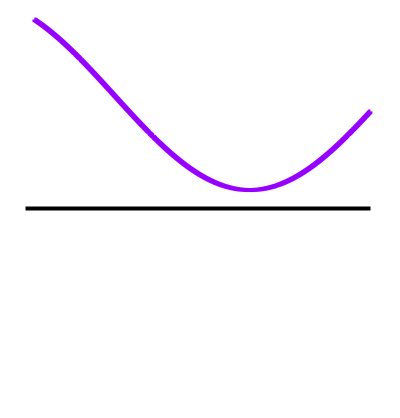
\includegraphics[height=3cm]{trichotomy-1}
  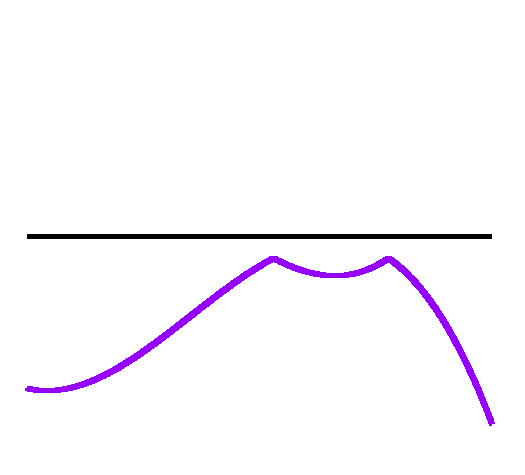
\includegraphics[height=3cm]{trichotomy-2}
  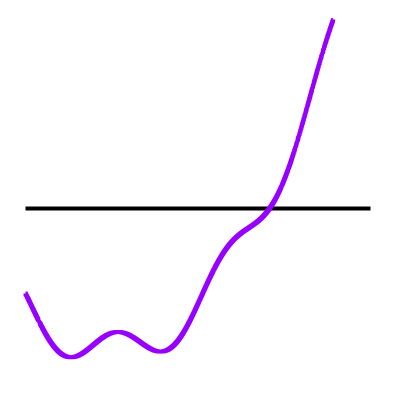
\includegraphics[height=3cm]{trichotomy-3}
  \caption{\label{fig:trichotomy} Three examples for what the topos~$\Sh(X)$
  each believes to be a single real number, where the base space~$X$ is the
  unit interval. (a) A positive real number. (b) A negative real number. (c) A
  number which is neither negative nor zero nor positive. Externally speaking,
  there is no covering of the unit interval by open subsets on which the
  depicted function~$a$ is either everywhere negative, everywhere zero or everywhere
  positive.}
\end{figure}


\subsection{Real functions} Let~$(f_x)_{x \in X}$ be a continuous family of
continuous real-valued functions; that is, each of the individual
functions~$f_x : \RR \to \RR$ should be continuous and moreover the map~$\RR
\times X \to \RR, (a,x) \mapsto f_x(a)$ should be continuous.
From the point of view of~$\Sh(X)$, this family looks like a single continuous
function~$f : \RR \to \RR$.

The internal statement that~$f(-1) < 0$ means that~$f_x(-1) < 0$ for all~$x \in
X$, and similarly so for being positive. More generally, if~$a$ and~$b$ are
continuous functions~$X \to \RR$ (hence real numbers from the internal point of
view), the internal statement~$f(a) < b$ means that~$f_x(a(x)) < b(x)$ for
all~$x \in X$.

The internal statement that~$f$ possesses a zero, that is, that there exists a
number~$a$ such that~$f(a) = 0$, means that all the functions~$f_x$ each
possess a zero and that moreover, these zeros can locally be picked in a
continuous fashion. More precisely, this statement means that there is an open
covering~$X = \bigcup_i U_i$ such that, for each~$i$, there is a continuous
function~$a : U_i \to \RR$ such that~$f_x(a(x)) = 0$ for all~$x \in U_i$. (On
overlaps~$U_i \cap U_j$, the zero-picking functions~$a$ need not agree.)

From these observations we can deduce that the intermediate value theorem of
basic analysis does in general not hold in~$\Sh(X)$ and hence does not allow
for an intuitionistic proof. This theorem states: ``If~$f : \RR \to \RR$
is a continuous function such that~$f(-1) < 0$ and~$f(1) > 0$, there exists a
number~$a$ such that~$f(a) = 0$.'' The external meaning of this statement is
that in any continuous family~$(f_x)_x$ of continuous functions with~$f_x(-1) <
0$ and~$f_x(1) > 0$ for all~$x \in X$, it's locally possible to pick zeros of
the family in a continuous fashion. Figure~\ref{fig:ivt} shows a counterexample
to this claim.


% \begin{document}

\section{XXX ... infinitesimal numbers ...}

The idea of \emph{infinitesimal numbers} -- numbers which lie between~$-1/n$
and~$1/n$ for any natural number~$n$ -- has a long and rich history. They are
not part of today's standard setup of the reals, but they are still intriguing
as calculational tools and as a device to bring mathematical intuition and
mathematical formalism closer together.

For instance, employing numbers~$\varepsilon$ such that~$\varepsilon^2 = 0$, we can
compute derivatives blithely as follows, without requiring the notion of
limits:
\begin{align*}
  (x + \varepsilon)^2 - x^2 &= x^2 + 2x\varepsilon + \varepsilon^2 - x^2 = 2x\varepsilon \\
  (x + \varepsilon)^3 - x^3 &= x^3 + 3x^2\varepsilon + 3x\varepsilon^2 + \varepsilon^3 - x^3 = 3x^2\varepsilon
\end{align*}
In each case, the derivative is visible as the coefficient of~$\varepsilon$ in
the result. A further example is from geometry: Having a nontrivial
set~$\Delta$ of infinitesimal numbers available allows us to define a
\emph{tangent vector} to a manifold~$M$ to be a map~$\gamma : \Delta \to M$. This
definition precisely captures the intuition that a tangent vector is an
infinitesimal curve.


\subsection{Hyperreal numbers} There are several ways for introducing
infinitesimals into rigorous mathematics. One is Robinson's \emph{nonstandard
analysis}, where we enlarge the field~$\RR$ of real numbers to a
field~$^\star\RR$ of \emph{hyperreal numbers} by means of a non-principal
ultrafilter.

The hyperreals contain an isomorphic copy of the ordinary reals as the
so-called \emph{standard elements}, and they also contain infinitesimal numbers
and their inverses, transfinite numbers, and support a powerful \emph{transfer
principle}: Any statement which doesn't refer to standardness is true for the
hyperreals if and only if it is true for the ordinary reals.

In the ``if'' direction, the transfer principle is useful for importing
knowledge about the ordinary reals in the hyperreal realm. For instance,
addition of hyperreals is commutative because addition of reals is.
By the ``only if'' direction, a theorem established for the hyperreals also
holds for the ordinary reals. In this way, the infinitesimal numbers of
nonstandard analysis can be viewed as a convenient fiction, generating a
conservative extension of the usual setup of mathematics.

However, the realization of this fiction crucically rests on a non-principal
ultrafilter, whose existence requires principles which go beyond the means of
Zermelo--Fraenkel set theory~\textsc{zf}.\footnote{A hyperreal number is
represented by an infinite sequence~$(x_0,x_1,x_2,\ldots)$ of ordinary real
numbers. For instance, the sequence~$(1,1,1,\ldots)$ represents the hyperreal
version of the number~$1$, the sequence~$(1,\frac{1}{2},\frac{1}{3},\ldots)$
represents an infinitesimal number and its inverse~$(1,2,3,\ldots)$ represents
a transfinite number.
%
The sequence~$(1,1,1,\ldots)$ is deemed positive, and so is~$(-1,1,1,1,\ldots)$,
which differs from the former only in finitely many places. But
should~$(1,-1,1,-1,\ldots)$ be deemed positive or negative? Whatever the
answer, our decision has consequences for other sequences. For
instance~$(-1,1,-1,1,\ldots)$ should be assigned the opposite sign
and~$(\tan(1),\tan(-1),\tan(1),\tan(-1),\ldots)$ the same.
%
A non-principal ultrafilter is a set-theoretic gadget which fixes all such
decisions once and for all in a coherent manner. Having such an ultrafilter
available, a sequence~$(x_0,x_1,x_2,\ldots)$ is deemed positive if and only if
the set~$\{i \in \NN \,|\, x_i > 0\}$ is part of the ultrafilter.}
Non-principal ultrafilters cannot be described in explicit terms, and
they are also not at all canonical structures: \textsc{zfc} proves that there
are~$2^{2^{\aleph_0}}$ many~\cite{pospisil:ultrafilters}.

A practical consequence of this non-constructivity is that it can be hard to
unwind proofs which employ hyperreal numbers to direct proofs, and even where
possible there is no general procedure for doing so.


\subsection{Topos-theoretic alternatives to the hyperreal numbers} Topos theory
provides several constructive alternatives for realizing infinitesimals.
One such is ``cheap nonstandard analysis'' by Terence Tao~\cite{tao:cheap-nsa}
and is related to Robinson's nonstandard analysis like potential infinity is
related to actual infinity. Instead of appealing to the axiom of choice to
obtain a completed ultrafilter, cheap nonstandard analysis constructs larger
and larger approximations to an ideal ultrafilter on the go.

The following section presents the basics of \emph{synthetic differential
geometry}~\cite{kock:sdg,kock:new-methods}. This is a further topos-theoretic
approach to infinitesimals which is suited to illustrate the philosophy of toposes
as lenses. Its stated goal is to devise a rigorous context in which the
writings of Sophus Lie, who freely employed infinitesimals in his seminal work
on differential geometry, can be effortlessly interpreted, staying close to the
original.


\subsection{XXX ...}



\printbibliography

\end{document}


Outline:


Stuff that should be mentioned:

* Andrej's realizability in the real world
* Cauchy vs. Dedekind numbers (physical quantities, ...)
* Syntactical vs. semantical interpretation
* phone call analogy
* detailed explanation of the pretty picture; analogy with "inner models"
  of set theory
* quick overview of the several aspects of toposes (maybe at the end,
  as an outlook?)
* enrichment of platonism debate (find better term for this!)
* uncovering further relations between objects
* allowing a switch of perspective
* applications in mathematical practice
* int. logic as common denominator
* arbitrariness of the "standard axioms"
* models of ZF yield toposes (models of ETCS), including a quick discussion of
  equivalence
* what giving up classical logic actually amounts to in practice
* examples in Spec(A), "reifying all the individual localizations into a
  single coherent entity which can be reasoned about as if it were a single
  ring"
* importance of having an adapted language
* SDG (infinitesimals are well-studied in philosophy of mathematics)
* quick remark on the internal language being based on types instead of sets
* reference to Bohr topos approach
* Source https://plato.stanford.edu/entries/category-theory/ for relevant
  literatur
* the internal language as a generalized modal operator

* use the phrase "very rich and very deep" (or similarly) about set theory
* PA doesn't have models
* Sven(?)

Send to Georg.
Also Giuseppe Cammarata.

Mention forcing
